\chapter{链路感知的选择性语义通信}
\label{rq2:chapter}

\section{引言}
前一章从网络层研究了无人机节点的路由与功率控制，使有限能量能够支持较为持久的数据传输。当无人机承担巡检、目标搜索和现场态势理解等任务时，仅保证数据可以到达接收端仍不足以说明通信资源得到了有效利用。不同节点拍摄的图像既可能相互补充，也可能包含大量重复内容；同一图像中的大部分像素还可能与当前任务无关。如果所有节点都按照固定频率上传完整观测，有限带宽会同时被关键证据和无关信息占用。因而，在链路能够承载消息的基础上，还需要回答哪些消息值得传输。

以多架无人机共同判断现场某处是否具备通行条件为例，一架无人机可以看清入口，却不能观察入口后的障碍物；另一架无人机能够观察道路局部，但受到遮挡，难以判断障碍物与通道的位置关系。两者给出的局部结论可能并不一致。决策中心需要获得与当前查询相关的证据，并据此修正判断。在较短通信窗口内，中心可能只来得及接收若干条标签或简短陈述，难以接收全部图像与完整解释。通信决策因此包含三个相互关联的问题：选择证据来源，确定消息粒度，以及判断何时停止继续通信。

视觉语言模型能够将局部图像组织为标签、置信度、信念分布和自然语言摘要，为上述选择提供了统一的语义接口。然而，模型给出的高置信度并不必然意味着证据可靠；来自相似视角的多个高置信判断也可能重复同一错误。与此同时，消息越长，其传输时间通常越长，在短暂链路窗口内完成交付的概率越低。仅依据语义相关性选择消息，会忽略消息的可达性；仅依据链路质量选择消息，则可能优先传输容易到达但无法改变判断的证据。任务导向通信需要同时衡量消息的语义收益和传输代价\cite{semantic-communications-jsac,semantic-communications-survey}。

针对这一问题，本章提出链路感知选择性语义通信方法 EviComRL。该方法利用冻结视觉语言模型构造离线语义轨迹，将昂贵的语义提取过程与通信策略学习分离；在有限通信预算下，通过结构化候选编码、发送方可靠性特征和历史上下文，学习逐步选择消息的策略。算法采用带动作掩码的近端策略优化，在训练奖励中联合考虑信念质量、分类结果、消息长度、时延和链路风险。实验以 VQAv2/COCO 派生的五级证据可见性任务为载体，考察方法在不同视角数量、通信预算、链路条件和消息粒度下的表现，并通过网络结构与可靠性特征消融分析各组成部分的作用。

\section{协同语义通信系统模型}
\label{rq2:sec:model}
\subsection{局部观测与五级证据可见性任务}
考虑由 $N$ 个局部观测节点和一个决策中心构成的协同系统。局部节点集合记为 $\mathcal N=\{1,\ldots,N\}$，决策中心用 $c_0$ 表示。一次任务由完整场景图像 $I_k$ 和视觉查询 $q_k$ 确定，各节点只能观察该图像的局部区域 $o_{i,k}$。这一设定将无人机视角受限的特点转化为可重复的局部证据获取过程：不同裁剪区域对应不同观测覆盖，不额外改变视觉语言模型的参数。

VQAv2 提供图像及其相关问题，COCO 提供包含多类目标与复杂背景的自然场景图像\cite{vqa-v2,coco}。本章利用这些样本构造问题相关的证据可见性判断任务。给定查询，模型判断当前视角中是否包含支持回答的视觉证据，标签空间定义为
\begin{equation}
\mathcal Y=\{\text{清晰可见},\text{大部分可见},\text{不确定},\text{大部分遮挡},\text{完全遮挡}\}.
\label{rq2:eq:labels}
\end{equation}
五个标签从证据充分到证据缺失排列，但训练中的分类损失与评价指标仍按五类任务计算。某一局部区域可以包含查询中提及的目标，却不足以支持判断其属性或关系，因此这里的可见性与单纯的目标是否出现并不相同。视觉问答中的关注区域与证据定位研究也表明，问题的语义内容会改变模型需要观察的图像区域\cite{where-to-look-vqa,vqa-hat,gqa}。

冻结视觉语言模型根据完整图像和查询生成参考标签 $y_k^*$，局部节点则仅根据各自裁剪图像生成证据。$y_k^*$ 是全图模型提供的弱监督参考，用于训练奖励和离线评价。局部策略的输入不包含这一标签，也不包含依靠该标签计算的正确性。因而，本章准确率反映局部证据通信后的判断与全图参考判断之间的一致程度，不能直接解释为原始 VQA 自然语言答案的准确率。

节点 $i$ 的局部证据表示为
\begin{equation}
e_{i,k}=\left(y_{i,k},p_{i,k},u_{i,k},q_{i,k}^{\mathrm{obs}},\ell_{i,k},r_{i,k},\bm b_{i,k}\right),
\label{rq2:eq:evidence}
\end{equation}
其中 $y_{i,k}$ 为局部预测标签，$p_{i,k}$ 为置信度，$u_{i,k}$ 为不确定性，$q_{i,k}^{\mathrm{obs}}$ 表示观测质量，$\ell_{i,k}$ 为裁剪区域，$r_{i,k}$ 为文字摘要。信念向量 $\bm b_{i,k}\in\mathbb R^5$ 满足 $b_{i,k}^{y}\geq0$ 和 $\sum_y b_{i,k}^{y}=1$，其熵为
\begin{equation}
H(\bm b_{i,k})=-\sum_{y\in\mathcal Y}b_{i,k}^{y}\log\max\{b_{i,k}^{y},\varepsilon\}.
\label{rq2:eq:entropy}
\end{equation}
置信度刻画当前结论的集中程度，熵描述整个类别分布的不确定性，观测质量则反映图像证据本身是否清晰、完整。这些量来源不同，不能简单相互替代。例如，模型可能在低质量裁剪上给出集中但错误的分布，因此策略还需要利用多节点间的相对关系识别证据来源。

主设置采用不具有本地图像的盲决策中心，其初始信念为 $\bm b_{c_0,k}^{0}=\bm u$，其中 $\bm u=(1/5,\ldots,1/5)$。这一设置使最终决策依赖实际被选中的跨节点消息。所有节点的原始证据只用于形成候选及其可观测特征，中心不会直接将未选择的节点信念作为已接收证据加入最终判断。候选元数据被视为任务初始化时可获得的调度信息，其采集成本不在本章消息预算内单独计量。

\subsection{多粒度消息及其链路代价}
对同一局部证据构造四种消息模式
\begin{equation}
\mathcal C=\{\mathrm{label},\mathrm{claim},\mathrm{summary},\mathrm{full}\}.
\label{rq2:eq:modes}
\end{equation}
标签模式保留最紧凑的类别信息；陈述模式描述与查询相关的主要判断；摘要模式提供支持判断的局部语义依据；完整模式保留较充分的结构化证据。消息 $m=(i,j,c)$ 指定发送方、接收方与模式，其长度记为 $T_m$。同一节点的不同模式共享观测来源，因而它们并不是相互独立的视觉证据。选择多个来自同一节点的模式可能加强已有结论，也可能占用本应分配给其他视角的预算。

一般通信空间允许节点间定向传输，原始候选规模至多为 $N(N-1)|\mathcal C|$。在盲中心主设置中，候选被转换为面向中心的发送方--模式组合，因此实际选择重点是证据来源和语义粒度，候选规模约为 $N|\mathcal C|$。这种汇聚结构符合中心需要整合多架无人机局部证据的任务需求，也便于在同一接收目标下比较不同消息的收益。

令节点间距离为 $d_{ij}$，带宽状态和链路质量因子分别为 $\eta_{ij}^{\mathrm{bw}}$ 和 $\eta_{ij}^{\mathrm{link}}$。本章采用与距离和链路状态有关的速率代理模型
\begin{equation}
v_{ij}=\left(v_{\max}e^{-\zeta d_{ij}}+v_{\min}\right)
\max\{0.05,\eta_{ij}^{\mathrm{bw}}\eta_{ij}^{\mathrm{link}}\}.
\label{rq2:eq:rate}
\end{equation}
将每个 token 的平均字节数记为 $b_{\mathrm{tok}}$，则消息大小、传输时延与发送能量分别为
\begin{equation}
B_m=b_{\mathrm{tok}}T_m,\qquad
L_m=\frac{B_m}{v_{ij}},\qquad E_m=P_{\mathrm{tx}}L_m.
\label{rq2:eq:cost}
\end{equation}
该模型用于给不同长度、不同链路条件的消息提供一致的比较尺度。它描述语义层决策面对的通信代价，不承担对完整无人机无线协议栈的复现。

链路可用窗口记为 $D_m$。当消息传输时间接近可用窗口长度时，小幅链路波动就可能改变消息能否及时到达。采用平滑映射描述这一变化：
\begin{equation}
p_m^{\mathrm{del}}=\frac{1}{1+\exp[-(D_m-L_m)/\tau]},\qquad
R_m^{\mathrm{drop}}=1-p_m^{\mathrm{del}}.
\label{rq2:eq:delivery}
\end{equation}
其中温度参数 $\tau$ 控制窗口边界附近的变化幅度。该关系同时作用于消息长度和链路条件：在其他因素不变时，长消息的 $L_m$ 较大，送达概率下降；较好的带宽和链路质量则缩短传输时间。策略因此能够区分“内容丰富”与“能够及时产生作用”这两个不同属性。

\subsection{冻结语义轨迹与中心信念更新}
冻结轨迹包括全图参考标签、局部证据、各模式消息、消息长度、链路代价以及接收方信念更新信息。原始节点间轨迹通过冻结模型离线计算消息后信念，其增量可表示为
\begin{equation}
\Delta\bm b_{i\to j,k}^{c}
=\kappa_c\left[\mathcal U(o_{j,k},e_{j,k},m_{i\to j,k}^{c})-\bm b_{j,k}^{0}\right].
\label{rq2:eq:raw_update}
\end{equation}
其中 $\mathcal U$ 为固定的语义更新模块，$\kappa_c$ 为消息模式的融合强度。轨迹生成完成后，策略训练和测试均只读取保存的结果，避免反复调用大模型造成的生成随机性和计算开销。不同通信方法由此面对相同的局部证据与链路元数据。

盲决策中心没有初始视觉观测。为了使局部节点信息在中心先验上具有统一的增量定义，主设置将发往中心的消息重新表示为
\begin{equation}
\begin{aligned}
\Delta\bm b_{i\to c_0,k}^{c}&=\kappa_c(\bm b_{i,k}-\bm u),\\
(\kappa_{\mathrm{label}},\kappa_{\mathrm{claim}},\kappa_{\mathrm{summary}},\kappa_{\mathrm{full}})
&=(0.22,0.42,0.62,0.78).
\end{aligned}
\label{rq2:eq:center_update}
\end{equation}
该处理使不同语义模式在同一标签空间中形成不同强度的证据输入。其含义是以离线节点信念和预设融合强度模拟语义消息对中心的作用，长消息的具体贡献仍需通过模式对照实验评价。

选择消息 $m_t$ 后，接收方按如下规则更新信念：
\begin{equation}
\bm b_j^{t+1}=\mathcal P\!\left[\bm b_j^t+
\left(p_{m_t}^{\mathrm{del}}\right)^\alpha\Delta\bm b_{m_t}\right].
\label{rq2:eq:belief_update}
\end{equation}
算子 $\mathcal P$ 先将负分量截断为零，再对所有分量归一化；若截断后的总质量为零，则返回均匀分布。主设置取 $\alpha=0.5$，以送达概率的平方根对信念增量折扣。$\alpha=0$ 表示取消额外的增量折扣，$\alpha=1$ 表示按送达概率线性缩放。本章将在实验中分别报告主设置和取消折扣的对照，避免把不同更新规则的数值混合为同一结果。

该更新是固定轨迹上的信念融合规则，并非对每次分组成功或失败进行抽样后的真实接收过程。多条增量依次作用时，截断与归一化也会使后续消息的边际收益依赖已接收内容。消息顺序、已选集合和当前信念因此共同决定最终结果，这构成采用序列决策方法的依据。

\begin{figure}[htbp]
\centering
\begin{tikzpicture}[x=1mm,y=1mm,>=Stealth,
  font=\fontsize{9bp}{11.5bp}\selectfont,
  ewbox/.style={draw,line width=.45pt,align=center,text width=38mm,
    minimum height=10mm,inner sep=1mm},
  ewarrow/.style={->,line width=.55pt},
  ewnote/.style={align=center,inner sep=.4mm,fill=white}]
\path[use as bounding box] (0,1) rectangle (148,-42);
\node[ewnote] at (74,-1) {离线构造：参考标签仅用于训练与评价};
\node[ewbox] (image) at (25,-9.5) {完整图像与查询\\局部视角裁剪};
\node[ewbox] (vlm) at (74,-9.5) {冻结视觉语言模型\\标签、信念与摘要};
\node[ewbox] (trace) at (123,-9.5) {冻结语义轨迹\\消息、代价与增量};
\node[ewbox] (candidate) at (123,-25.5) {成本敏感检索\\链路感知重排序};
\node[ewbox] (policy) at (74,-25.5) {可靠性与历史编码\\掩码策略网络};
\node[ewbox] (action) at (25,-25.5) {发送消息或停止\\中心信念与资源更新};
\draw[ewarrow] (image) -- (vlm);
\draw[ewarrow] (vlm) -- (trace);
\draw[ewarrow] (trace) -- (candidate);
\draw[ewarrow] (candidate) -- (policy);
\draw[ewarrow] (policy) -- (action);
\draw[ewarrow] (action.south) -- (25,-34.5) -- (74,-34.5) -- (policy.south);
\node[ewnote] at (49.5,-34.5) {信念、历史与剩余预算};
\node[ewnote] at (74,-40) {训练：代理预热与 PPO\qquad 测试：固定参数执行};
\end{tikzpicture}

\bicaption{冻结语义轨迹与选择性通信策略的整体流程}{Overall workflow of frozen semantic traces and selective communication}
\label{rq2:fig:workflow}
\end{figure}

\subsection{约束条件与优化目标}
设 $\mathcal S_t$ 为第 $t$ 步之前已经选择的消息集合，$U_t=\sum_{m\in\mathcal S_t}T_m$ 为累计消息长度，$n_j^t$ 为接收方已接收的消息数量，$e_i^t$ 为发送方剩余能量状态。通信预算为 $T_{\mathrm{bud}}$，最大通信步数为 $H$，单个接收方容量为 $C_j$。合法消息需要满足
\begin{equation}
\begin{aligned}
m&\notin\mathcal S_t, & U_t+T_m&\leq T_{\mathrm{bud}},\\
p_m^{\mathrm{del}}&\geq p_{\min}, & n_j^t&<C_j,\\
e_i^t&\geq e_{\min}, & t&<H.
\end{aligned}
\label{rq2:eq:constraints}
\end{equation}
其中剩余能量门限是候选发送的可行性检查，发送后按 $e_i^{t+1}=\max\{0,e_i^t-E_m\}$ 更新。消息级截止时间违约通过风险和代价项体现。本章没有把所有消息的累计时延再限制在一个单独的任务硬截止时间内，这一区别将在下一章的交付控制模型中进一步处理。

决策中心的最终预测和信念质量分别定义为
\begin{equation}
\hat y_k=\arg\max_{y\in\mathcal Y} b_{c_0,k}^{\tau_k,y},\qquad
Q_k= b_{c_0,k}^{\tau_k,y_k^*},
\label{rq2:eq:quality}
\end{equation}
其中 $\tau_k\leq H$ 为实际停止步数。优化目标是在上述可行域中选择策略 $\pi$，使最终任务质量与通信成本形成适当折中：
\begin{equation}
\max_{\pi}\ \mathbb E_{k,\pi}\!\left[
\begin{aligned}
&\lambda_Q Q_k+\lambda_A\mathbf1\{\hat y_k=y_k^*\}
-\beta_T\frac{U_{\tau_k}}{T_{\mathrm{bud}}}\\
&\hspace{1em}-\beta_L\sum_{m\in\mathcal S_{\tau_k}}L_m
-\beta_R\sum_{m\in\mathcal S_{\tau_k}}R_m^{\mathrm{drop}}
\end{aligned}\right].
\label{rq2:eq:objective}
\end{equation}
该问题具有有限候选、可变长度动作序列和非线性信念更新。精确枚举所有可行消息顺序的代价随候选规模和通信步数快速增长。EviComRL 采用候选检索缩小动作空间，再通过强化学习近似优化序列收益。

\section{可靠性与历史感知的通信策略}
\label{rq2:sec:algorithm}
\subsection{候选检索与链路感知重排序}
直接将全部候选输入网络会扩大动作空间，也会使大量低价值动作参与早期探索。EviComRL 首先进行成本敏感检索。令 $C_{ij}^{\mathrm{conf}}$ 表示发送方与接收方预测之间的冲突程度，$C_{ij}^{\mathrm{comp}}$ 表示由观测区域重合程度得到的互补性，$b_c$ 为模式强度相关项，则初筛分数为
\begin{equation}
S_1(m)=\frac{H(\bm b_j^0)+C_{ij}^{\mathrm{conf}}+C_{ij}^{\mathrm{comp}}+q_i^{\mathrm{obs}}+0.2b_c}
{(T_m/T_{\mathrm{bud}}+L_m+\varepsilon)(1+R_m^{\mathrm{drop}})}.
\label{rq2:eq:retrieval}
\end{equation}
接收方熵较高意味着尚有改善判断的空间；不同预测与互补视角提示消息可能补充当前证据；消息长度、时延和风险则降低其价值密度。这一分数仅使用通信前可获得的信息，不需要知道消息是否会修正为参考标签。

对初筛得到的前 $K$ 个候选，进一步采用语义收益与链路代价的加权分数重排序：
\begin{equation}
\begin{aligned}
S_2(m)={}&H(\bm b_j^0)+C_{ij}^{\mathrm{conf}}+C_{ij}^{\mathrm{comp}}+q_i^{\mathrm{obs}}
+0.6\mathbf1\{j=c_0\}\\
&+0.4p_m^{\mathrm{del}}+0.2\eta_{ij}^{\mathrm{link}}+0.1\eta_{ij}^{\mathrm{bw}}
-0.7T_m/T_{\mathrm{bud}}-0.2L_m-0.4R_m^{\mathrm{drop}}.
\end{aligned}
\label{rq2:eq:rerank}
\end{equation}
取排序最高的 $M$ 个候选构成该回合的固定候选集合。主设置 $K=32$、$M=16$。后续通信步骤不重新调用语义模型，也不重新扩充候选池，而是根据最新信念和预算更新候选特征及可行性。检索决定哪些证据进入策略视野，策略则决定这些证据是否值得在当前时刻发送，两者承担不同职责。

在全部消息均发往盲中心的主设置中，式\eqref{rq2:eq:rerank}中的中心偏好是候选间相同的常数，因此不会改变排序。保留这一项有助于统一一般节点间通信接口，但其收益不能在单中心汇聚任务中单独体现。对应消融实验也应依据这一结构解释，而不能预期每一个可配置权重都会产生可观测的性能差异。

\subsection{发送方可靠性特征与状态表示}
仅将模型置信度作为可靠性指标，难以区分真实清晰观测与过度自信的错误判断。本章在候选中补充五类可观测可靠性特征。对节点 $i$ 的信念从大到小排序为 $b_i^{(1)}\geq b_i^{(2)}\geq\cdots$，定义
\begin{equation}
\begin{aligned}
\bm r_i&=[r_{i,1},r_{i,2},r_{i,3},r_{i,4},r_{i,5}],\\
r_{i,1}&=b_i^{(1)},\quad r_{i,2}=b_i^{(1)}-b_i^{(2)},\quad
r_{i,3}=H(\bm b_i)/\log5,\\
r_{i,4}&=\frac{\sum_{v\ne i}\mathbf1\{q_v^{\mathrm{obs}}<q_i^{\mathrm{obs}}\}}{\max(1,|\mathcal V|-1)},\quad
r_{i,5}=\frac{\sum_v q_v^{\mathrm{obs}}\mathbf1\{\hat y_v=\hat y_i\}}{\sum_v q_v^{\mathrm{obs}}+\varepsilon}.
\end{aligned}
\label{rq2:eq:reliability}
\end{equation}
这里 $\mathcal V$ 为任务中的节点集合，包含观测质量为零的盲中心。前两项刻画分布峰值及第一、第二类别之间的间隔，第三项刻画整体不确定性，后两项分别表示节点观测质量的相对排名和质量加权共识支持度。相较于只统计赞同节点的数量，质量加权共识降低了多个低质量视角对判断的影响。不过，共识只能作为策略输入；若多个节点共同产生错误，较高共识仍不能保证结论正确。

每条候选采用 41 维特征，具体组成如表\ref{rq2:tab:features}所示。全局状态为 11 维向量：剩余预算比例、中心最大信念、当前步数比例、已用预算比例、累计时延、累计能量以及中心五维信念。中心最大信念是策略可观察的确定性程度，与仅能在训练阶段计算的 $Q_k$ 不同。

\begin{table}[htbp]
\centering
\bicaption{候选消息的结构化特征组成}{Structured features of each candidate message}
\label{rq2:tab:features}
\begin{tabularx}{\textwidth}{l r X}
\toprule
特征类别 & 维数 & 具体内容\\
\midrule
发送方与证据关系 & 6 & 置信度、不确定性、观测质量、接收方熵、预测冲突、观测互补性\\
语义粒度 & 4 & 四种消息模式的独热编码\\
通信与历史状态 & 10 & 消息长度、时延、窗口、送达概率、丢包风险、已选状态、中心标记、链路质量、带宽因子、能量代价\\
节点信念 & 15 & 发送方、接收方和决策中心各自的五维信念\\
可靠性信息 & 5 & 信念峰值、类别间隔、归一化熵、观测质量排名、加权共识\\
候选存在标记 & 1 & 区分真实候选与补齐固定长度的空白项\\
\bottomrule
\end{tabularx}
\end{table}

将第 $t$ 步输入表示为 $s_t=(X_t,\bm g_t,\bm\mu_t)$，其中 $X_t\in\mathbb R^{M\times41}$ 为候选特征矩阵，$\bm g_t\in\mathbb R^{11}$ 为全局状态，$\bm\mu_t$ 为动作掩码。环境完整状态还包括所有节点信念、已选集合、接收次数和剩余能量。网络输入是对这些量的结构化观测，固定轨迹上的更新过程则由环境保存的消息增量决定。

\subsection{结构化候选编码与历史上下文融合}
候选消息对应有向通信关系，发送方、接收方、语义模式与链路状态具有不同含义。网络先用共享编码器将每个完整候选映射为基础表示 $\bm h_m^0\in\mathbb R^d$，再分别编码各类子特征：
\begin{equation}
\bm h_m^0=f_{\mathrm{cand}}(\bm x_m),\quad
\bm z_t=f_g(\bm g_t),\quad
\bm v_m^{a}=f_a(\bm x_m^{a}),\ a\in\{s,r,c,l,b,q\}.
\label{rq2:eq:encoders}
\end{equation}
六个结构分支分别处理发送方、接收方、模式、链路、三方信念及可靠性信息。基础编码器采用两层全连接网络，其余分支采用全连接层与双曲正切激活。主设置隐藏维数 $d=64$。不同候选共享参数，使网络可以在固定上限内处理不同数量的实际候选，不需要为某一发送方单独设置一组网络权重。

已选消息会改变后续动作的价值，策略需要保留历史选择。令 $e_m$、$s_m^t$ 和 $c_m$ 分别为候选存在标记、已选标记与中心接收标记，定义两种上下文表示：
\begin{equation}
\bar{\bm h}_t^{\mathrm{sel}}=
\frac{\sum_m e_ms_m^t\bm h_m^0}{\max(1,\sum_m e_ms_m^t)},\qquad
\bar{\bm h}_t^{\mathrm{ctr}}=
\frac{\sum_m e_mc_m\bm h_m^0}{\max(1,\sum_m e_mc_m)}.
\label{rq2:eq:history}
\end{equation}
已选历史使用候选存在性而非当前动作合法性作为汇聚条件。这样，已经发送而被动作掩码禁止再次选择的消息仍保留在历史上下文中。中心上下文则描述与最终决策直接相关的候选集合。两种上下文都随候选的动态特征变化，能够将过去选择与当前接收需求联系起来。

将基础表示、六个结构分支、已选上下文、中心上下文和全局状态拼接，形成关系表示
\begin{equation}
\bm u_m=f_{\mathrm{rel}}\!\left[
\bm h_m^0,\bm v_m^s,\bm v_m^r,\bm v_m^c,\bm v_m^l,
\bm v_m^b,\bm v_m^q,\bar{\bm h}_t^{\mathrm{sel}},\bar{\bm h}_t^{\mathrm{ctr}},\bm z_t\right].
\label{rq2:eq:relation}
\end{equation}
该结构显式利用消息关系与候选集合上下文，不要求构造全体候选两两之间的注意力矩阵。通过门控残差将其与基础编码融合：
\begin{equation}
\bm a_m=\sigma\!\left(W_a[\bm h_m^0,\bm u_m,\bm z_t]+\bm b_a\right),\qquad
\bm h_m=\bm h_m^0+\bm a_m\odot\bm u_m.
\label{rq2:eq:gate}
\end{equation}
门控偏置初始取负值，使训练初期以基础特征为主，随后根据梯度逐步调整结构分支的作用强度。其目的在于避免新增分支在随机初始化时大幅扰动候选表示。

\begin{figure}[htbp]
\centering
% Matches GraphHistoryActorCriticNet and Eqs. (encoders)--(policy).
% Repeated tensor names denote reuse, not additional encoders or observations.
\begin{tikzpicture}[
  x=1mm,y=1mm,>=Stealth,
  font=\fontsize{9bp}{11.5bp}\selectfont,
  enbox/.style={draw,line width=.45pt,fill=white,align=center,inner sep=1mm},
  enencoder/.style={enbox,text width=16.5mm,minimum height=13mm},
  encontext/.style={enbox,text width=32mm,minimum height=14mm},
  enarrow/.style={->,line width=.55pt},
  enwire/.style={line width=.45pt},
  entag/.style={fill=white,inner sep=.5mm}
]
\path[use as bounding box] (0,0) rectangle (148,-145);

\node[enbox,text width=143mm,minimum height=7mm] (enx) at (74,-3.5)
  {候选特征 $X_t\in\mathbb R^{M\times41}$\qquad 主设置 $M=16$，共享隐藏维数 $d=64$};
\draw[enwire] (enx.south) -- (74,-10);
\draw[enwire] (11,-10) -- (137,-10);

\node[enencoder] (enbase) at (11,-19.5)
  {基础编码\\\mbox{$41{\to}d{\to}d$}\\$\bm h_m^0$};
\node[enencoder] (ensender) at (32,-19.5)
  {发送方\\$3\to d$\\$\bm v_m^s$};
\node[enencoder] (enreceiver) at (53,-19.5)
  {接收方\\$2\to d$\\$\bm v_m^r$};
\node[enencoder] (enmode) at (74,-19.5)
  {语义模式\\$4\to d$\\$\bm v_m^c$};
\node[enencoder] (enlink) at (95,-19.5)
  {链路代价\\$7\to d$\\$\bm v_m^l$};
\node[enencoder] (enbelief) at (116,-19.5)
  {三方信念\\$15\to d$\\$\bm v_m^b$};
\node[enencoder] (enreliability) at (137,-19.5)
  {可靠性\\$5\to d$\\$\bm v_m^q$};
\foreach \name/\x in {enbase/11,ensender/32,enreceiver/53,enmode/74,enlink/95,enbelief/116,enreliability/137}
  \draw[enarrow] (\x,-10) -- (\name.north);

% The six structural branches are concatenated at the relation encoder.
\foreach \name/\x in {ensender/32,enreceiver/53,enmode/74,enlink/95,enbelief/116,enreliability/137}
  \draw[enwire] (\name.south) -- (\x,-29);
\draw[enwire] (32,-29) -- (146.5,-29) -- (146.5,-65);
\foreach \x in {53,74,95,116,137}
  \fill (\x,-29) circle (.45mm);

% Both contexts pool the base encoding, not the gate-enriched candidates.
\draw[enwire] (enbase.south) -- (11,-31) -- (80,-31);
\fill (34,-31) circle (.45mm);
\draw[enwire] (11,-31) -- (3,-31) -- (3,-86);
\fill (11,-31) circle (.45mm);

\node[encontext] (enselected) at (34,-42)
  {已选历史汇聚\\权重 $e_m s_m^t$ 的均值\\$\bar{\bm h}_t^{\mathrm{sel}}$};
\node[encontext] (encenter) at (80,-42)
  {中心上下文汇聚\\权重 $e_m c_m$ 的均值\\$\bar{\bm h}_t^{\mathrm{ctr}}$};
\node[enbox,text width=39mm,minimum height=14mm] (englobal) at (124,-42)
  {全局输入 $\bm g_t\in\mathbb R^{11}$\\全局编码 $f_g:11\to d$\\$\bm z_t$};
\draw[enarrow] (34,-31) -- (enselected.north);
\draw[enarrow] (80,-31) -- (encenter.north);

\foreach \name/\x in {enselected/34,encenter/80,englobal/124}
  \draw[enwire] (\name.south) -- (\x,-52.5);
\draw[enwire] (34,-52.5) -- (124,-52.5);
\fill (80,-52.5) circle (.45mm);
\draw[enarrow] (78,-52.5) -- (78,-57);

\node[enbox,text width=126mm,minimum height=16mm] (enrelation) at (78,-65)
  {关系拼接与编码 $f_{\mathrm{rel}}$\\
   $[\bm h_m^0,\bm v_m^s,\bm v_m^r,\bm v_m^c,\bm v_m^l,
     \bm v_m^b,\bm v_m^q,\bar{\bm h}_t^{\mathrm{sel}},\bar{\bm h}_t^{\mathrm{ctr}},\bm z_t]$\\
   $10d\to d\to d$，输出 $\bm u_m$};
\draw[enarrow] (146.5,-65) -- (enrelation.east);
\draw[enarrow] (3,-65) -- (enrelation.west);
\fill (3,-65) circle (.45mm);

\node[enbox,text width=116mm,minimum height=16mm] (engate) at (78,-86)
  {门控残差融合\\
   $\bm a_m=\sigma\!\left(W_a[\bm h_m^0,\bm u_m,\bm z_t]+\bm b_a\right)$\\
   $\bm h_m=\bm h_m^0+\bm a_m\odot\bm u_m$};
\draw[enarrow] (enrelation.south) -- (engate.north);
\draw[enarrow] (3,-86) -- node[entag] {$\bm h_m^0$} (engate.west);
% Named input reuses the global encoding shown above, avoiding a crossing wire.
\draw[enarrow] (146.5,-86) -- node[above,font=\fontsize{9bp}{11.5bp}\selectfont] {$\bm z_t$} (engate.east);

\draw[enwire] (engate.south) -- (78,-98);
\draw[enwire] (42,-98) -- (119,-98);
\node[entag] at (78,-98) {$\bm h_m$};

\node[enbox,text width=74mm,minimum height=19mm] (enactor) at (42,-112.5)
  {\textbf{Actor}：消息头与停止头\\
   $\ell_m=f_{\mathrm{act}}[\bm h_m,\bm z_t,\bar{\bm h}_t^{\mathrm{sel}},\bar{\bm h}_t^{\mathrm{ctr}}]$\\
   $\ell_0=f_{\mathrm{stop}}[\bm z_t,\bar{\bm h}_t^{\mathrm{sel}},\bar{\bm h}_t^{\mathrm{ctr}}]$\\
   消息：$4d\to d\to1$；停止：$3d\to d\to1$};
\node[enbox,text width=50mm,minimum height=19mm] (encritic) at (119,-112.5)
  {\textbf{Critic}：价值估计\\
   合法候选的 $\bm h_m$ 掩码均值\\
   拼接 $\bm z_t,\bar{\bm h}_t^{\mathrm{sel}},\bar{\bm h}_t^{\mathrm{ctr}}$\\
   $4d\to d\to1$};
\draw[enarrow] (42,-98) -- (enactor.north);
\draw[enarrow] (119,-98) -- (encritic.north);

\node[enbox,text width=54mm,minimum height=12mm] (enpolicy) at (42,-134)
  {非法消息置极小分数，Softmax\\
   $\pi_\theta(a\mid s_t),\quad a\in\{0,1,\ldots,M\}$};
\draw[enarrow] (enactor.south) -- (enpolicy.north);
\node[enbox,text width=17mm,minimum height=10mm] (enmask) at (86.5,-134)
  {合法掩码\\$\bm\mu_t$};
\draw[enarrow] (enmask.west) -- (enpolicy.east);
\draw[enarrow] (enmask.north) -- (86.5,-112.5) -- (encritic.west);
\node[align=center] (envalue) at (119,-134) {价值 $V_\psi(s_t)$};
\draw[enarrow] (encritic.south) -- (envalue.north);

\node[align=center,text width=143mm] at (74,-142.8)
  {同名张量表示结果复用；历史汇聚保留已选消息；停止动作始终可用。};
\end{tikzpicture}

\bicaption{可靠性与历史感知的掩码策略网络}{Reliability- and history-aware masked policy network}
\label{rq2:fig:network}
\end{figure}

消息动作与停止动作的分数分别为
\begin{equation}
\begin{aligned}
\ell_m&=f_{\mathrm{act}}[\bm h_m,\bm z_t,\bar{\bm h}_t^{\mathrm{sel}},\bar{\bm h}_t^{\mathrm{ctr}}],\\
\ell_0&=f_{\mathrm{stop}}[\bm z_t,\bar{\bm h}_t^{\mathrm{sel}},\bar{\bm h}_t^{\mathrm{ctr}}].
\end{aligned}
\label{rq2:eq:logits}
\end{equation}
动作空间为 $\{0,1,\ldots,M\}$，其中零表示停止通信。根据式\eqref{rq2:eq:constraints}将非法消息分数置为极小值，再作归一化：
\begin{equation}
\pi_\theta(a\mid s_t)=
\frac{\mu_t(a)\exp(\ell_a)}{\sum_{v=0}^M\mu_t(v)\exp(\ell_v)}.
\label{rq2:eq:policy}
\end{equation}
停止动作始终可用。当所有通信动作非法时，策略直接停止；当仍有可发送消息时，网络比较其后续收益与当前停止收益，自行决定是否继续。价值网络将合法候选的掩码均值、历史上下文、中心上下文和全局表示联合输入，估计当前状态的后续回报。

\subsection{奖励塑形与代理预热}
单步奖励以中心信念变化为基础。记 $Q_t=b_{c_0}^{t,y^*}$，则选中消息 $m$ 后的即时奖励为
\begin{equation}
\begin{aligned}
r_t={}&2.5(Q_{t+1}-Q_t)-0.015\frac{T_m}{T_{\mathrm{bud}}}
-0.01L_m-0.003E_m\\
&-0.03R_m^{\mathrm{drop}}-0.03\mathbf1\{L_m>D_m\}.
\end{aligned}
\label{rq2:eq:reward}
\end{equation}
在终止时追加
\begin{equation}
r_{\mathrm{end}}=Q_{\tau}+0.5\mathbf1\{\hat y=y^*\}
+0.5\left(b_{c_0}^{\tau,y^*}-\max_{y\ne y^*}b_{c_0}^{\tau,y}\right)
-0.005\frac{U_{\tau}}{T_{\mathrm{bud}}}.
\label{rq2:eq:terminal}
\end{equation}
即时信念增益提供较密集的学习信号，终止正确性和类别间隔将最终分类表现纳入训练目标。消息成本则使策略在语义收益较小时倾向停止。参考标签仅用于这些训练回报的计算，测试阶段的动作选择仍依据可观测状态和已训练参数。

在随机策略下，大量初始动作可能只产生负代价，停止动作也可能过早占据较大概率。为提高初始样本利用率，本章在 PPO 之前加入一步展望代理预热。对于训练状态 $s$，比较立即停止与执行一个合法消息后停止的回报：
\begin{equation}
\widehat U(s,a)=
\begin{cases}
r_{\mathrm{end}}(s),&a=0,\\
r(s,a)+r_{\mathrm{end}}(s'),&a\ne0\text{ 且未终止},\\
r(s,a),&a\ne0\text{ 且已终止}.
\end{cases}
\label{rq2:eq:proxy}
\end{equation}
对所有合法动作取最大值生成预热目标 $a^*$。若执行动作本身已包含终止奖励，不再次重复计入。代理动作只在训练轨迹上构造，并不作为测试阶段访问未知结果的手段。网络采用交叉熵损失 $\mathcal L_{\mathrm{pre}}=-0.2\log\pi_\theta(a^*\mid s)$ 训练三轮，随后进入 PPO。该初始化提供“何时值得发送”的初始偏好，长期序列权衡仍由后续强化学习优化。

\subsection{PPO 优化及执行过程}
PPO 通过限制一次更新中新旧策略的概率比，降低策略变化过大引起的训练波动\cite{ppo}。设采样时策略为 $\pi_{\theta_{\mathrm{old}}}$，定义
\begin{equation}
\begin{aligned}
\rho_t(\theta)&=\frac{\pi_\theta(a_t\mid s_t)}{\pi_{\theta_{\mathrm{old}}}(a_t\mid s_t)},\\
\mathcal L_{\mathrm{clip}}&=
-\mathbb E_t\min\left\{\rho_t(\theta)\widehat A_t,
\operatorname{clip}[\rho_t(\theta),1-\epsilon,1+\epsilon]\widehat A_t\right\}.
\end{aligned}
\label{rq2:eq:ppo}
\end{equation}
状态、动作掩码、旧动作概率与旧价值估计均在采样时保存，在同一批样本的多轮更新中保持不变。尤其是动作掩码对应采样时的预算和已选状态，不能在更新期间使用另一状态的合法性重新计算概率比。

优势采用广义优势估计\cite{gae}。对回合末尾取 $V(s_{\tau})=0$，反向计算
\begin{equation}
\delta_t=r_t+\gamma V_\psi(s_{t+1})-V_\psi(s_t),\qquad
\widehat A_t=\delta_t+\gamma\lambda\widehat A_{t+1},\qquad
\widehat R_t=\widehat A_t+V_\psi(s_t).
\label{rq2:eq:gae}
\end{equation}
总损失为
\begin{equation}
\mathcal L=\mathcal L_{\mathrm{clip}}+
0.5\mathbb E_t(V_\psi(s_t)-\widehat R_t)^2
-0.01\mathbb E_t\mathcal H[\pi_\theta(\cdot\mid s_t)].
\label{rq2:eq:loss}
\end{equation}
价值损失提供回报基线，熵项维持适度探索。每轮采样后进行四轮小批量更新，并采用梯度范数裁剪。训练过程中依据验证集上的确定性平均回报保留参数，测试集仅用于最终评价。主设置采用普通任务采样，不启用类别平衡重采样。

\begin{algorithm}[htbp]
\caption{EviComRL 的策略训练过程}
\label{rq2:alg:training}
\begin{algorithmic}[1]
\Require 冻结训练轨迹 $\mathcal D_{\mathrm{tr}}$、验证轨迹 $\mathcal D_{\mathrm{val}}$，候选上限 $M$ 与预算 $T_{\mathrm{bud}}$
\Ensure 通信策略参数 $\theta^*$
\State 将局部证据映射到盲中心，初始化共享编码器、策略网络与价值网络
\State 在训练轨迹中枚举一步展望动作，按式\eqref{rq2:eq:proxy}生成代理目标
\State 执行三轮代理交叉熵预热
\For{每轮 PPO 训练}
  \State 清空采样缓存
  \For{训练集中的每个任务}
    \State 检索并重排序候选，初始化中心信念、已选集合和资源状态
    \While{回合尚未结束}
      \State 更新结构化特征和合法动作掩码
      \State 从 $\pi_\theta$ 采样动作，记录旧动作概率和状态价值
      \State 执行动作，更新信念与成本，保存奖励和终止标记
    \EndWhile
  \EndFor
  \State 计算优势与回报，最小化式\eqref{rq2:eq:loss}并裁剪梯度
  \State 在验证集按最大动作概率执行策略
  \If{验证平均回报提高}
    \State 保存当前参数为 $\theta^*$
  \EndIf
\EndFor
\State \Return $\theta^*$
\end{algorithmic}
\end{algorithm}

测试阶段不再更新网络参数，也不再枚举依赖训练参考标签的代理目标。每步执行概率最大的合法动作，发送消息后更新信念与资源统计，直到网络选择停止或可行消息耗尽。该过程将候选筛选、状态更新和终止判断连接为一个有限长度的通信决策闭环。

\subsection{计算复杂度与方法适用范围}
设原始候选数量为 $A$，隐藏维数为 $d$。直接排序实现的候选筛选复杂度为 $O(A\log A)$；在主设置下，$A$ 随局部节点数量近似线性增长。共享候选编码和各结构分支的前向计算复杂度为 $O(Md^2)$，历史与中心上下文汇聚为 $O(Md)$。每个回合至多执行 $H$ 步，策略推理复杂度因而为 $O(A\log A+HMd^2)$。算法不对全部候选排列逐一求解，也不在推理时调用大模型评价每个备选动作。

代理预热需要在训练状态枚举合法动作，其一次目标构造约为 $O(M)$ 次环境更新。该开销发生在离线训练阶段，且轨迹更新只涉及短信念向量与资源计数。实际部署仍需承担局部语义提取的计算开销，本章所给策略复杂度主要描述语义证据已经得到之后的通信调度部分。

方法利用了固定标签空间、小规模候选集合及语义轨迹可重复回放等条件。对于开放式长文本回答，消息的贡献可能不能用五维信念增量完整表示；对于收到确认之前无法知道交付状态的系统，发送者还需要维护对接收端状态的估计。这两类因素分别对应语义表达能力与传输反馈机制的进一步扩展，本章重点研究前者固定时的选择性通信问题。

\section{实验设置与评价方法}
\label{rq2:sec:setup}
\subsection{数据与实现参数}
实验使用 3000 条 VQAv2/COCO 派生语义轨迹，语义提取模型为冻结的 Qwen3-VL-8B-Instruct。每条轨迹包含同一场景的局部节点证据和消息候选，主设置采用 9 个局部视角及一个盲决策中心。任务按标签分层划分为约 60\% 的训练集、20\% 的验证集和20\% 的测试集，主实验测试任务数为600。这里按任务样本划分数据；来自同一图像的不同问题不额外作为图像组整体划分，因此该实验测量的是当前任务划分下的策略泛化表现。

表\ref{rq2:tab:parameters}列出主要参数。完整跨条件实验包含28个配置，覆盖主设置、节点数量、预算、通信步数、链路条件、轨迹规模、消息模式和模块消融，各条件使用同一套方法与评价流程。该组实验采用一个随机种子和80轮训练。发送方可靠性特征另以三个随机种子开展成对消融，均使用3000条任务轨迹和80轮训练；其均值与标准差单独报告，不与单种子主表混合。

\begin{table}[htbp]
\centering
\bicaption{EviComRL 的主要实验参数}{Main experimental parameters of EviComRL}
\label{rq2:tab:parameters}
\begin{tabular}{ll ll}
\toprule
参数 & 取值 & 参数 & 取值\\
\midrule
局部视角数 & 9 & 通信预算 & 120 token\\
候选上限 $M$ & 16 & 初筛数量 $K$ & 32\\
最大步数 $H$ & 8 & 接收容量 & 3 条消息\\
最低送达概率 & 0.45 & 增量折扣指数 $\alpha$ & 0.5\\
隐藏维数 $d$ & 64 & 候选/全局维数 & 41/11\\
学习率 & $10^{-3}$ & PPO 裁剪阈值 & 0.2\\
回报折扣 $\gamma$ & 0.96 & GAE 参数 $\lambda$ & 0.95\\
小批量大小 & 32 & 梯度范数上限 & 0.5\\
代理预热轮次 & 3 & PPO 训练轮次 & 80\\
平均字节/token & 4 & 发送功率 & 1.5 W\\
速率参数 $v_{\max}$ & 1000 byte/s & $v_{\min}$ & 10 byte/s\\
距离衰减系数 $\zeta$ & 0.01 & 窗口温度 $\tau$ & 0.04 s\\
\bottomrule
\end{tabular}
\end{table}

冻结轨迹用于控制语义生成差异，所有对比方法共享同一批局部证据、消息代价、候选上限和动作合法性约束。超参数与模型参数的选择依据训练和验证过程完成，测试阶段保持固定。实验不计入语义模型推理、飞行推进和候选元数据收集的能量；时延与能量指标表示本章消息模型下的通信代价。

\subsection{对比方法与评价指标}
对比方法包括三类。第一类为基础通信策略：NoComm 不发送消息，Random 随机选择合法候选，FullComm 在预算和接收容量内尽可能发送候选，TokenGreedy 优先选择短消息。由于接收容量和候选顺序的限制，FullComm 并不一定消耗最多 token，也不代表交换全部原始图像。

第二类为单步排序策略。Greedy 按语义收益与通信代价的比值选取候选，LearnRank 使用固定加权收益评分，SemanticOnly 主要考虑语义属性，LinkOnly 主要考虑可靠性与代价，ContextualBandit 则在任务上下文下学习单步动作偏好。这里 LearnRank 是当前实验中的加权排序参照，不将其描述为已训练的深度排序模型。

第三类为协同感知思想的轨迹适配方法与网络结构对照。Where2Comm-Trace 基于置信度和空间互补性选择信息，How2Comm-Trace 同时考虑协作收益、链路条件与重复接收代价，其思想分别来自空间置信图通信和实用协同感知方法\cite{where2comm,how2comm}。本章对它们统一使用语义消息轨迹和相同约束，比较的是相关通信原则在当前任务中的适配表现，不能据此推断原论文端到端感知系统的相对优劣。PPO-MLP 保留同样的输入与训练流程，将结构化关系分支替换为共享候选多层感知机，用于检验网络结构的作用。

设测试集大小为 $n$，对每类 $y$ 统计真阳性 $\mathrm{TP}_y$、假阳性 $\mathrm{FP}_y$ 和假阴性 $\mathrm{FN}_y$，则准确率、平衡准确率和宏平均 F1 分别为
\begin{equation}
\begin{aligned}
\mathrm{Acc}&=\frac1n\sum_k\mathbf1\{\hat y_k=y_k^*\},\\
\mathrm{BAcc}&=\frac1{|\mathcal Y_+|}\sum_{y\in\mathcal Y_+}
\frac{\mathrm{TP}_y}{\mathrm{TP}_y+\mathrm{FN}_y},\\
\mathrm{MF1}&=\frac15\sum_{y\in\mathcal Y}
\frac{2\mathrm{TP}_y}{2\mathrm{TP}_y+\mathrm{FP}_y+\mathrm{FN}_y}.
\end{aligned}
\label{rq2:eq:metrics}
\end{equation}
其中 $\mathcal Y_+$ 为测试集中实际出现的类别，F1 分母为零时该类记零。类别数量不均衡时，仅预测常见类别也可能取得一定准确率，因此平衡准确率与宏平均 F1 对结果解释是必要的。

通信代价报告每任务平均通信 token 数、平均消息数、累计时延及风险。其中，通信 token 数先对单个任务内所选消息的长度求和，再对测试任务取平均，记为 $\bar T$。先对每个任务所选消息的送达概率求平均，再对任务求平均，记为 $\bar p^{\mathrm{del}}$；零通信任务的该项约定为1。有效信念质量与质量成本比定义为
\begin{equation}
Q_{\mathrm{eff}}=\bar Q\,\bar p^{\mathrm{del}},\qquad
\mathrm{QCR}=\frac{Q_{\mathrm{eff}}}
{1+\bar T/100+\bar L+0.2\bar E+\bar R^{\mathrm{drop}}+\bar D^{\mathrm{miss}}}.
\label{rq2:eq:qcr}
\end{equation}
有效信念质量是平均信念质量与平均送达概率的乘积，用于综合观察语义判断和链路条件；它不是逐次真实送达后的正确服务率。QCR 的分母包含常数1，NoComm 的数值因而有限，但低成本本身仍可能使其表现偏高，需要结合分类指标一并判断。

\section{实验结果与分析}
\label{rq2:sec:results}
\subsection{主设置下的推理质量与通信代价}
表\ref{rq2:tab:main}给出主设置结果。EviComRL 的准确率、平衡准确率和宏平均 F1 分别为58.17\%、53.05\%和50.58\%，均高于表中其他对比方法。相比 FullComm，准确率提高11.00个百分点，宏平均 F1 提高13.20个百分点，说明受限预算下根据任务状态进行选择，能够比按既定顺序发送候选更充分地利用有效证据。相比 ContextualBandit，准确率提高7.50个百分点，每任务平均通信量从69.24 token降至49.70 token，表明序列策略并非只依靠增加通信量获得质量提升。

\begin{table}[htbp]
\centering\small
\bicaption{主设置下不同通信方法的测试结果}{Test results of different communication methods under the main setting}
\label{rq2:tab:main}
\setlength{\tabcolsep}{3.2pt}
\begin{tabular}{lrrrrrr}
\toprule
方法 & Acc/\% & BAcc/\% & MF1/\% & \shortstack{每任务平均\\通信量/token} & $Q_{\mathrm{eff}}$ & QCR\\
\midrule
\textbf{EviComRL} & \textbf{58.17} & \textbf{53.05} & \textbf{50.58} & 49.70 & \textbf{0.3854} & 0.1780\\
PPO-MLP & 54.83 & 50.39 & 46.92 & 53.50 & 0.3757 & 0.1664\\
ContextualBandit & 50.67 & 51.49 & 40.49 & 69.24 & 0.3384 & 0.1267\\
FullComm & 47.17 & 47.68 & 37.38 & 31.71 & 0.3252 & 0.1814\\
SemanticOnly & 45.50 & 46.37 & 36.69 & 50.51 & 0.3240 & 0.1423\\
TokenGreedy & 44.67 & 47.75 & 35.59 & 27.00 & 0.2923 & 0.1708\\
How2Comm-Trace & 42.67 & 46.44 & 34.15 & 34.56 & 0.3086 & 0.1771\\
Where2Comm-Trace & 34.33 & 40.57 & 28.30 & 27.00 & 0.2657 & 0.1676\\
LearnRank & 34.17 & 40.31 & 28.75 & 27.00 & 0.2627 & 0.1645\\
NoComm & 32.67 & 20.00 & 9.85 & 0.00 & 0.2000 & 0.2000\\
Greedy & 31.83 & 39.82 & 26.99 & 27.00 & 0.2575 & 0.1629\\
Random & 31.33 & 36.85 & 26.92 & 44.33 & 0.2369 & 0.1123\\
LinkOnly & 25.17 & 36.10 & 22.93 & 27.00 & 0.2342 & 0.1491\\
\bottomrule
\end{tabular}
\end{table}

图\ref{rq2:fig:accuracy}进一步比较了各方法的准确率。NoComm 的平衡准确率为20\%，与均匀先验通过固定并列处理输出单一类别的行为一致。LinkOnly 的准确率低于 NoComm，说明接收容易传输的消息也可能使原有判断朝错误类别移动。SemanticOnly 优于仅看链路的策略，但其有效信念质量仍低于 EviComRL，表明语义属性需要与传输风险、后续通信空间共同考虑。

\begin{figure}[htbp]
\centering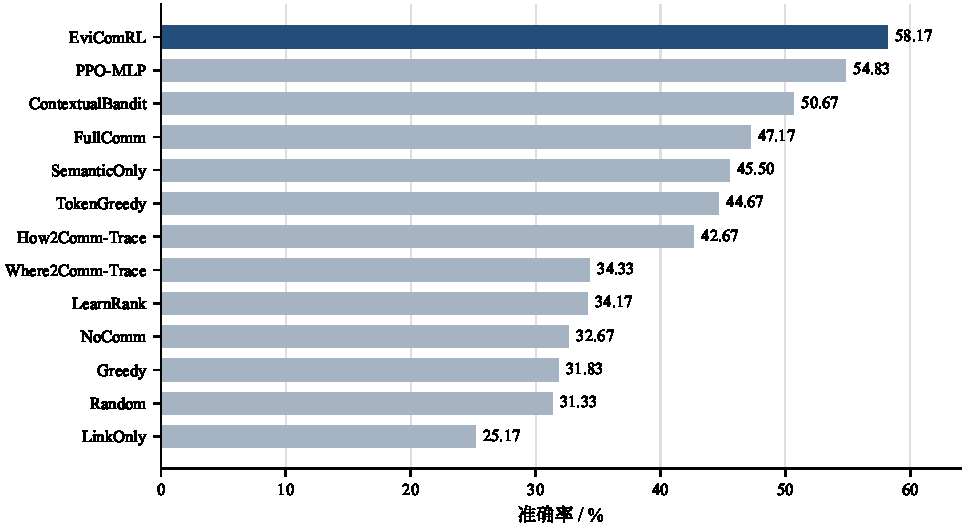
\includegraphics[width=.96\textwidth]{figures/rq2/main_accuracy.pdf}
\bicaption{主设置下的证据可见性分类准确率}{Evidence visibility classification accuracy under the main setting}
\label{rq2:fig:accuracy}
\end{figure}

图\ref{rq2:fig:tradeoff}展示质量与每任务平均通信量的关系。EviComRL 在约50 token处取得最高的有效信念质量，但其成本并非所有方法中最低。FullComm 与部分短消息方法位于更低成本区域，其中 FullComm 的 QCR 为0.1814，略高于 EviComRL 的0.1780。因此，主实验支持的是较高任务质量下的通信选择优势，并不意味着该策略在每一种质量成本权重下都最优。需要极端节省带宽时，可以采用更低预算或限制消息模式；需要更充分地形成中心信念时，则应允许策略使用部分较长消息。

\begin{figure}[htbp]
\centering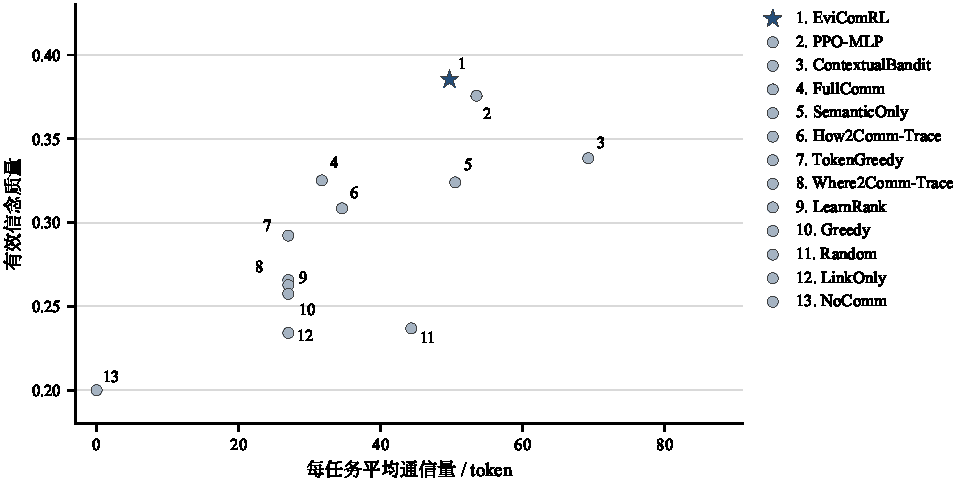
\includegraphics[width=.98\textwidth]{figures/rq2/quality_cost.pdf}
\bicaption{主设置下的有效信念质量与每任务平均通信量}{Effective belief quality versus average token expenditure per task under the main setting}
\label{rq2:fig:tradeoff}
\end{figure}

EviComRL 每个任务平均选择2.66条消息，低于8步上限，也低于接收容量3条。可见停止动作已经参与决策，最大步数并不等于实际发送次数。与 PPO-MLP 相比，结构化策略准确率提高3.33个百分点、宏平均 F1 提高3.65个百分点，同时使每任务平均通信量减少3.80 token。这一结果说明在同样输入与训练条件下，显式区分消息关系并汇聚历史上下文具有实际作用；它不等价于对每个结构分支分别完成了独立贡献证明。

\subsection{训练过程与策略收敛特征}
图\ref{rq2:fig:training}给出主设置80轮训练的平均回合回报。代理预热之后，策略已经具有初步的候选排序与停止偏好，PPO 在此基础上继续调整多步选择。回报在训练中仍有波动，这与随机动作探索、不同任务类别的收益差异以及更新中的小批量梯度有关。图中曲线表示训练采样回报，不能直接替代测试准确率，也不能以其中某个最高点作为最终测试结果。

\begin{figure}[htbp]
\centering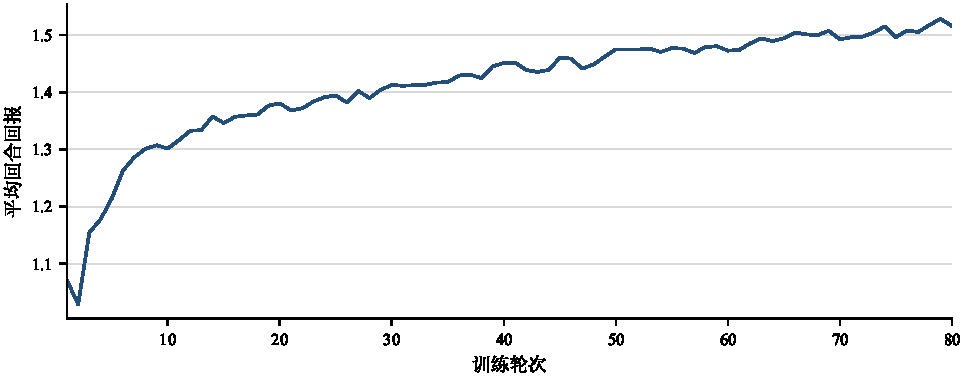
\includegraphics[width=.93\textwidth]{figures/rq2/training_curve.pdf}
\bicaption{主设置下 PPO 的训练回报变化}{PPO training returns under the main setting}
\label{rq2:fig:training}
\end{figure}

最终策略由验证集确定性回报选择，而不是简单使用最后一轮参数。该设置尤其适合有限轨迹上的训练：后期探索可能使采样回报暂时变化，但已获得的较好策略可以通过验证结果保留。另一方面，本章主条件实验仍只有一个训练随机种子，训练曲线体现的是该次优化过程的变化，不据此给出多次独立训练必然收敛到相同解的判断。

\subsection{局部视角数量的影响}
图\ref{rq2:fig:agents}考察3、6和9个局部视角。EviComRL 的准确率分别为35.00\%、53.83\%和58.17\%，宏平均 F1 分别为22.06\%、43.33\%和50.58\%。从3个视角增加到6个视角时，性能改善较大，表明通信策略无法弥补候选中本来就缺失的视觉证据。增加观测覆盖首先扩大了可获得信息的范围，再由策略筛选其中较可靠的部分。

\begin{figure}[htbp]
\centering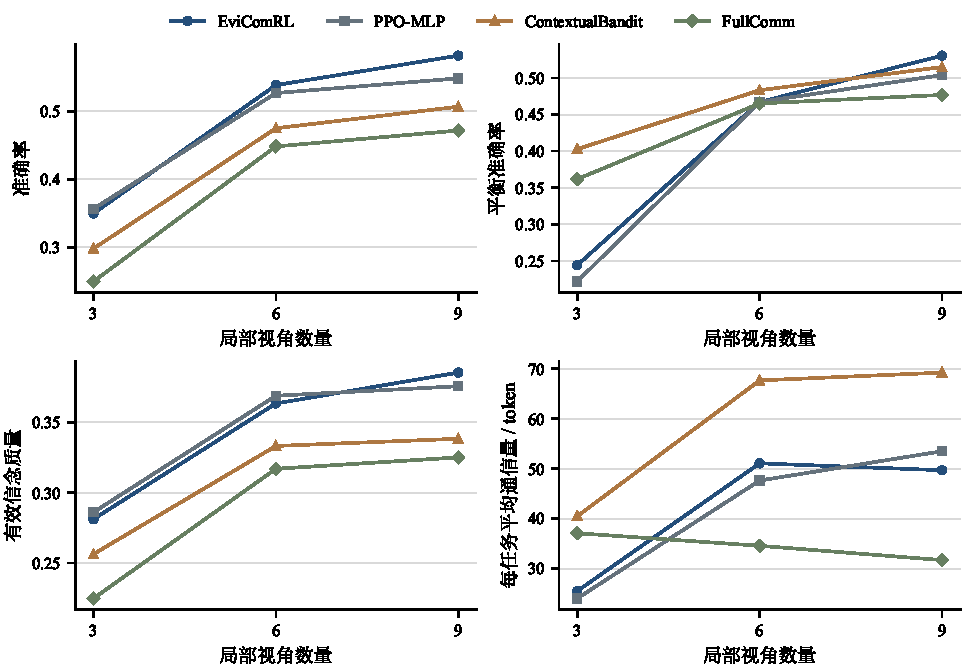
\includegraphics[width=\textwidth]{figures/rq2/agent_count.pdf}
\bicaption{不同局部视角数量下的质量与通信开销}{Quality and communication cost with different numbers of local views}
\label{rq2:fig:agents}
\end{figure}

由6个增加到9个视角后，EviComRL 的有效信念质量从0.3635提高到0.3854，而每任务平均通信量由51.08降至49.70 token。更多节点并未必然带来更多实际通信；较大的候选池使策略能够替换不可靠来源，以较少或较短的消息获得更好的证据组合。该组结果说明观测覆盖与消息筛选具有互补作用，但不能据此推断节点数继续增大时性能仍会单调提升。候选上限固定后，额外节点能否进入候选池也会受到检索质量的限制。

\subsection{通信预算与最大步数的影响}
图\ref{rq2:fig:budget}比较60、120、180和240 token预算。预算为60 token时，EviComRL 已达到58.00\%准确率，与120 token下的58.17\%接近，但宏平均 F1 由48.04\%提高到50.58\%，有效信念质量由0.3729提高到0.3854。这说明更多预算主要改善部分难例和信念分布，而非使所有任务的最终类别同时改变。

\begin{figure}[htbp]
\centering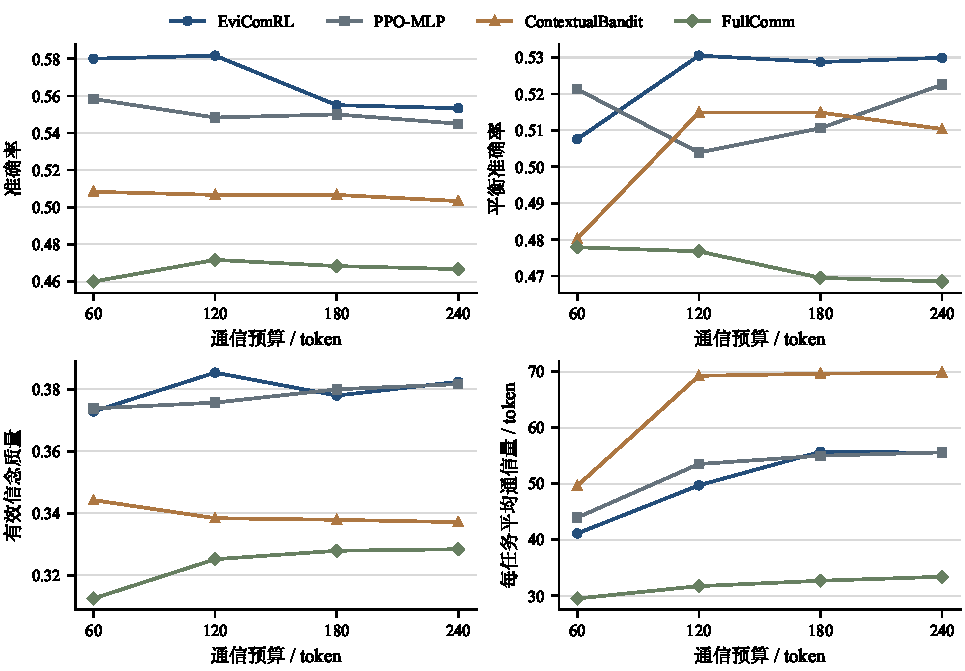
\includegraphics[width=\textwidth]{figures/rq2/budget.pdf}
\bicaption{不同通信预算下的性能变化}{Performance under different communication budgets}
\label{rq2:fig:budget}
\end{figure}

预算继续增至180和240 token后，准确率分别为55.50\%和55.33\%，没有延续上升趋势；实际每任务平均通信量仅约55.68和55.53 token，远低于预算上限。一方面，接收容量和停止决策限制了实际发送次数；另一方面，成本归一化随预算变化，较长消息进入候选排序的相对优势也会变化。增加预算同时改变可行域与学习时的质量成本权重，其效果不应被简单理解为给同一个固定策略添加更多消息。

\begin{figure}[htbp]
\centering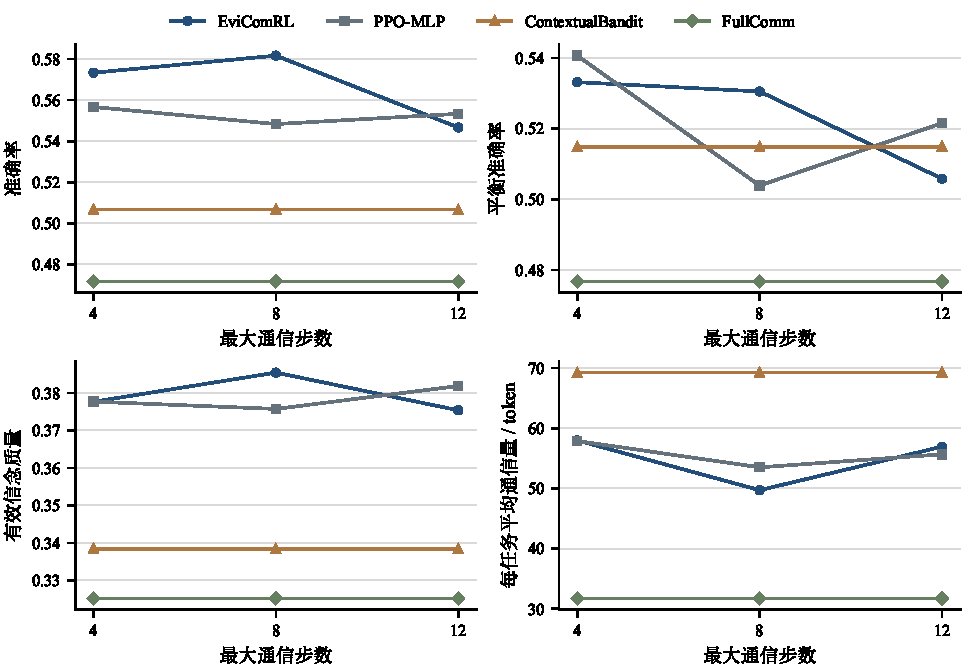
\includegraphics[width=\textwidth]{figures/rq2/max_steps.pdf}
\bicaption{最大通信步数对策略性能的影响}{Effect of the maximum number of communication steps}
\label{rq2:fig:steps}
\end{figure}

图\ref{rq2:fig:steps}进一步比较4、8和12步上限。8步设置准确率和有效信念质量较高，每任务平均通信量反而低于4步与12步设置。在单中心容量为3条的实验中，这些步数上限通常不会成为实际发送次数的主要限制，但步数归一化特征和训练过程仍会受到其影响。因而，该组实验更适合说明参数设置会改变策略偏好，不能解释为已经观察到12次真实消息交换带来的增益。主设置保留8步，以维持与全部对比方法一致的决策接口。

\subsection{链路可靠性及消息粒度的影响}
图\ref{rq2:fig:links}比较良好、中等和较差链路。较差链路通过降低送达概率、增大时延并降低链路状态因子构造，同时将最低送达门限调整为0.25，避免候选全部失去可行性。良好与中等条件的门限分别为0.35和0.45。因此，这些条件共同描述链路状态与可用候选范围的变化，不是只改变一个独立概率参数。

\begin{figure}[htbp]
\centering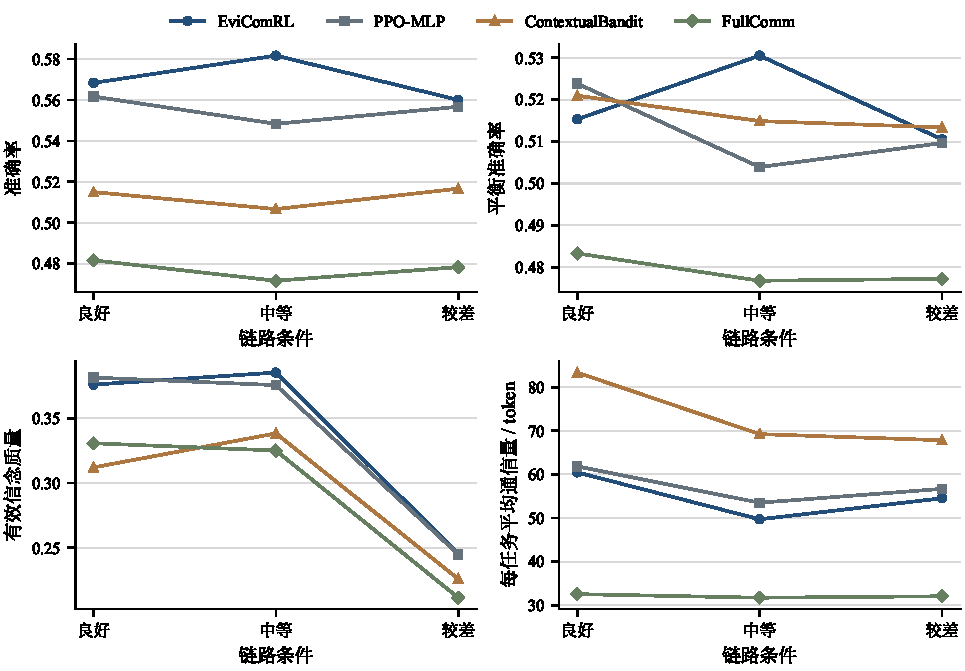
\includegraphics[width=\textwidth]{figures/rq2/link_profile.pdf}
\bicaption{不同链路条件下的推理质量与成本}{Inference quality and cost under different link conditions}
\label{rq2:fig:links}
\end{figure}

由中等链路变为较差链路时，EviComRL 的准确率从58.17\%下降到56.00\%，降幅不大，但有效信念质量从0.3854降至0.2453，QCR从0.1780降至0.0845。分类标签主要取决于最大信念分量，而有效质量还考虑信念集中程度和链路送达概率，因此两者对链路恶化的敏感程度不同。这一结果表明，通信研究不能仅报告最后的类别是否一致，还需要观察在不可靠链路下获得该判断的有效性与代价。

\begin{figure}[htbp]
\centering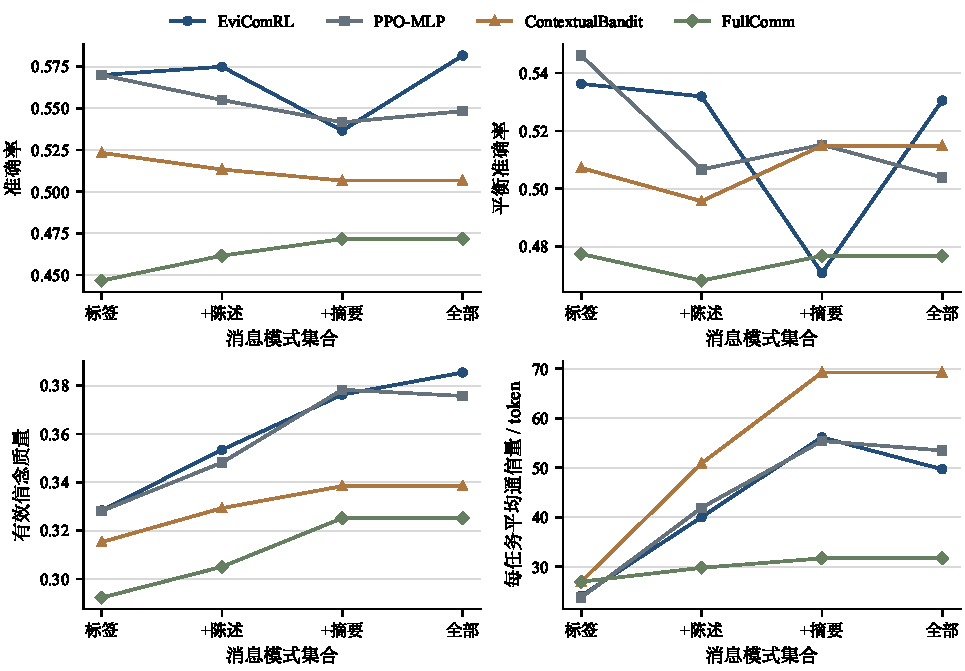
\includegraphics[width=\textwidth]{figures/rq2/message_modes.pdf}
\bicaption{可用语义消息模式对策略性能的影响}{Effect of available semantic message modes}
\label{rq2:fig:modes}
\end{figure}

图\ref{rq2:fig:modes}依次开放标签、陈述、摘要及全部模式。仅允许标签时，EviComRL 的准确率为57.00\%，平衡准确率为53.63\%，宏平均 F1 为51.26\%，每任务平均通信量仅24.14 token；全部模式下，准确率为58.17\%，每任务平均通信量为49.70 token，有效信念质量由0.3284提高到0.3854。短标签能够提供较强的类别判断信息，较丰富模式则在当前融合强度设定下增加信念质量，但未带来所有分类指标的一致改善。

这一现象与任务定义相符。五级可见性属于有限类别判断，简短标签已包含较直接的判别线索。较长摘要是否有额外价值，还取决于其是否提供了独立依据、是否能弥补其他视角的缺失以及是否增加了链路风险。该组实验支持让通信策略在不同粒度之间进行选择，并不支持把任一固定粒度推广为所有视觉推理任务的最优表达。

\subsection{轨迹规模及关键组成部分分析}
图\ref{rq2:fig:scale}比较500、1000和2000条轨迹的训练与评价结果。准确率分别为57.00\%、57.21\%和58.50\%，但平衡准确率与宏平均 F1 并未随规模单调变化。不同规模使用各自的数据子集和分层划分，较少样本条件下的少数类比例及具体测试难度更容易波动。因此，不能仅依据这三点拟合稳定的样本效率规律。该组结果表明较小轨迹集也能训练出有效策略，而跨规模泛化的精确结论仍需要固定测试集和重复训练进一步支持。

\begin{figure}[htbp]
\centering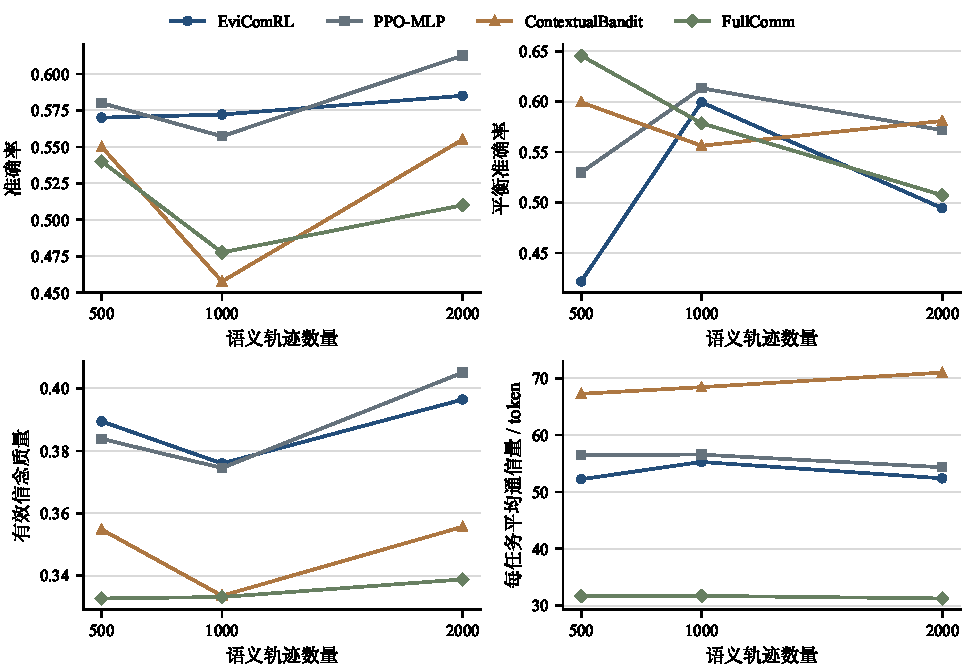
\includegraphics[width=\textwidth]{figures/rq2/trace_scale.pdf}
\bicaption{不同语义轨迹规模下的策略表现}{Policy performance with different semantic trace scales}
\label{rq2:fig:scale}
\end{figure}

图\ref{rq2:fig:ablation}与表\ref{rq2:tab:ablation}给出同一完整实验中的组件消融。取消重排序后，准确率从58.17\%降至51.00\%，宏平均 F1 从50.58\%降至43.51\%，是该组中较明显的退化。该消融直接使用轨迹顺序截取候选，因而同时去除了成本敏感检索和后续排序，说明高价值候选能否进入固定大小的动作集合对最终效果具有重要影响。

\begin{figure}[htbp]
\centering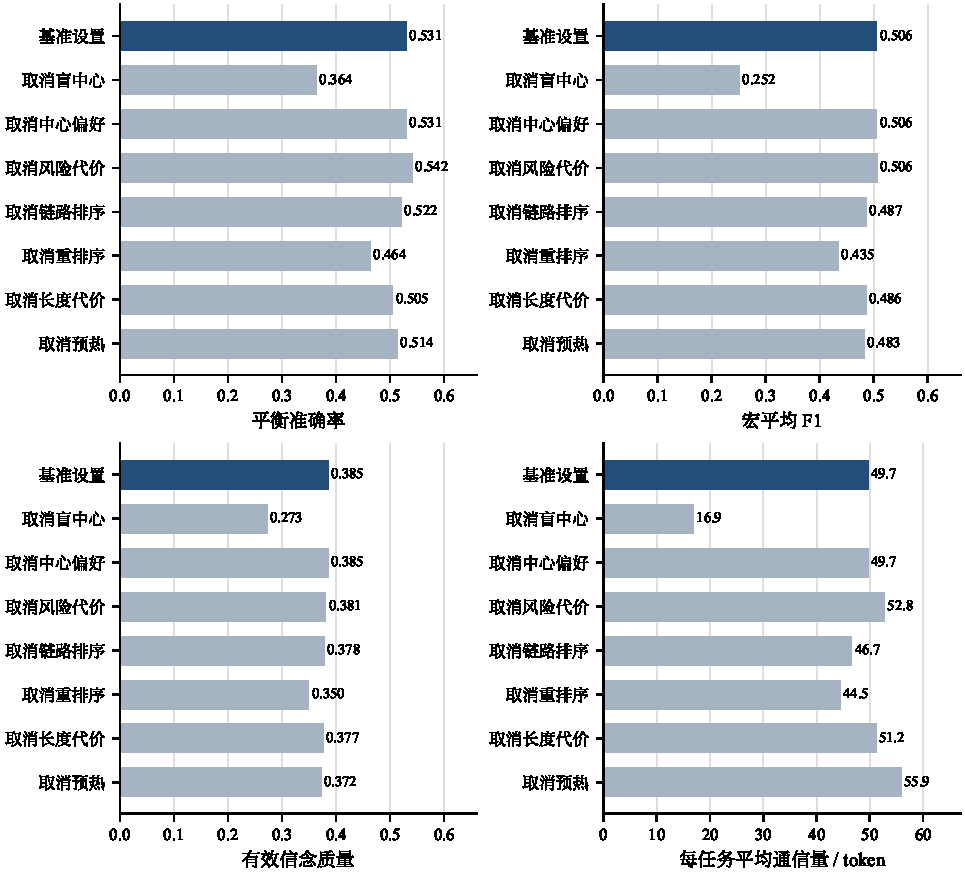
\includegraphics[width=\textwidth]{figures/rq2/ablation.pdf}
\bicaption{主要组成部分的消融结果}{Ablation results of the main components}
\label{rq2:fig:ablation}
\end{figure}

\begin{table}[htbp]
\centering\small
\bicaption{主要消融设置的分类质量与通信代价}{Classification quality and communication cost of main ablation settings}
\label{rq2:tab:ablation}
\begin{tabular}{lrrrrr}
\toprule
设置 & Acc/\% & BAcc/\% & MF1/\% & \shortstack{每任务平均\\通信量/token} & $Q_{\mathrm{eff}}$\\
\midrule
完整方法 & 58.17 & 53.05 & 50.58 & 49.70 & 0.3854\\
取消重排序 & 51.00 & 46.39 & 43.51 & 44.48 & 0.3500\\
取消链路排序 & 56.50 & 52.16 & 48.66 & 46.66 & 0.3785\\
取消中心偏好 & 58.17 & 53.05 & 50.58 & 49.70 & 0.3854\\
取消长度代价 & 56.33 & 50.55 & 48.61 & 51.20 & 0.3766\\
取消风险代价 & 56.67 & 54.17 & 50.62 & 52.80 & 0.3815\\
取消预热 & 55.00 & 51.41 & 48.33 & 55.94 & 0.3723\\
取消盲中心 & 27.17 & 36.41 & 25.19 & 16.90 & 0.2726\\
取消增量折扣 & 58.50 & 53.20 & 50.79 & 49.51 & 0.3957\\
\bottomrule
\end{tabular}
\end{table}

取消链路排序后，准确率与宏平均 F1 分别下降1.67和1.92个百分点，表明链路信息在候选形成阶段已产生作用。取消代理预热后，准确率降至55.00\%，每任务平均通信量增加至55.94 token，说明较好的初始化有助于策略识别有用发送动作并减少无效通信。取消风险代价时，平衡准确率略有提高，但准确率、有效信念质量和QCR下降；风险代价控制的是质量与链路成本的共同权衡，不保证每个分类指标均单独提高。

取消中心偏好与完整方法得到完全相同的结果，原因是主设置中全部候选都发往中心，该常数项不影响排序。取消盲中心则改变了接收端自身观测、候选方向与信念更新方式，应理解为任务接口对照，不能把其退化全部归因于某一个网络模块。取消增量折扣后，准确率小幅提高到58.50\%，有效信念质量提高到0.3957，说明平方根折扣在当前代理链路环境下仍存在保守性。该结果保留了折扣强度进一步校准的空间，也表明链路可靠性可以通过特征、掩码与成本项发挥作用，不必假定增量折扣越强越好。

为单独评价新增可靠性特征，本章进一步比较同一网络将五维可靠性输入置零与完整输入两种设置。三个随机种子结果汇总于表\ref{rq2:tab:reliability}，误差为样本标准差。两种设置使用相同训练规模、相同回报系数和相同训练轮次，区别仅在于可靠性特征是否可用。

\begin{table}[htbp]
\centering\small
\bicaption{发送方可靠性特征的三次重复实验}{Three-run comparison of sender reliability features}
\label{rq2:tab:reliability}
\begin{tabular}{lrrrr}
\toprule
设置 & Acc/\% & BAcc/\% & MF1/\% & \shortstack{每任务平均\\通信量/token}\\
\midrule
无可靠性特征 & $56.56\pm0.42$ & $50.70\pm0.34$ & $49.28\pm1.02$ & $53.43\pm2.06$\\
完整方法 & $58.50\pm0.88$ & $52.66\pm2.57$ & $51.48\pm3.15$ & $50.35\pm1.13$\\
\bottomrule
\end{tabular}
\end{table}

\begin{figure}[htbp]
\centering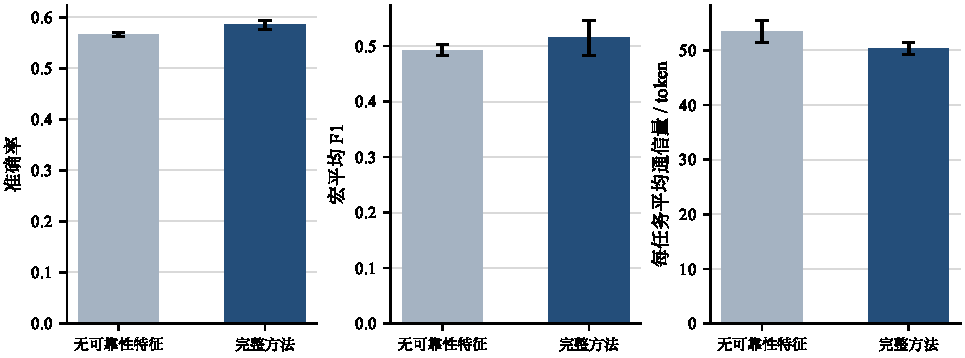
\includegraphics[width=\textwidth]{figures/rq2/reliability.pdf}
\bicaption{可靠性特征对分类质量和每任务平均通信量的影响}{Effect of reliability features on classification quality and average token expenditure per task}
\label{rq2:fig:reliability}
\end{figure}

完整方法的平均准确率由56.56\%提高到58.50\%，宏平均 F1由49.28\%提高到51.48\%，每任务平均通信量减少约3.08 token。图\ref{rq2:fig:reliability}表明该特征组在平均质量与成本上同时改善了结果，支持利用分布形状和多节点共识辅助识别可靠证据来源。平衡准确率与宏平均 F1 的重复实验波动仍较大，因此本章报告均值和标准差，不进一步宣称所有任务分布下均能获得固定幅度的提升。

\section{本章小结}
\label{rq2:sec:summary}
本章研究了局部视觉证据分散、消息长度受限和链路可靠性变化条件下的选择性语义通信问题。通过冻结视觉语言模型构造统一语义轨迹，将证据提取与通信策略训练分离；在中心信念、通信预算和消息可行域的共同约束下，设计成本敏感候选检索以及可靠性与历史感知的掩码策略网络，并以代理预热和PPO学习消息选择与停止行为。

实验结果表明，EviComRL 在主设置中取得58.17\%准确率，相比 FullComm 和 ContextualBandit 分别提高11.00和7.50个百分点，相比结构简化的 PPO-MLP 同时提高分类质量并减少每任务平均通信量。跨条件结果进一步说明，观测覆盖决定可获得证据的基础，预算与语义粒度影响质量成本折中，链路恶化则可能在最终类别变化不大时显著降低有效信念质量。可靠性特征的重复实验支持利用可观测信念形状和共识信息改善发送方选择。

本章的消息作用通过送达概率折扣和冻结增量回放表示。一次消息被选择后，环境立即更新中心信念，尚未区分发送完成、实际收到以及确认返回三个时刻。在确认延迟或丢失的条件下，发送端无法直接知道接收端究竟拥有哪部分证据；重复发送、等待确认与发送新证据之间的取舍也会影响时延和能量。下一章在本章的语义候选基础上进一步研究不完备反馈下的可靠交付与能量协同控制，使语义价值选择与实际传输过程形成连续的研究链条。
